\chapter{BDD frameworks in selected projects}
\label{chapter:projects}

This chapter illustrates how studied projects teams chose their implementation level BDD testing
framework to take in use for the project. The process is explained in detail with examples of JUnit tests
refactored into different BDD testing frameworks.

\section{How project teams chose their new testing framework}
\label{section:teams}
    Projects are denoted as \textbf{A} and \textbf{B}. Full description of projects can be found in section \ref{section:demographics} in the interview
    results. In brief, they both can be categorized as \textit{Spring Framework} projects. Project A is a \textit{Spring Boot} project, where
    most of the needed dependencies are bundled under Spring Boot configuration. Project B is a conventional Spring Framework project,
    where needed dependencies are added individually into build configuration.

    Both projects and their teams were first introduced to built proof of concept examples of \textbf{RSpec, Spock} and \textbf{Spectrum}
    in use for an example Java Spring Framework project. Some of these used examples can be found in chapter \ref{chapter:environment}.
    All my subjective pros and cons of these BDD testing frameworks versus JUnit were demonstrated. RSpec was stripped from the
    potential candidates from both project first, as it included a more complicated development and build environment configuration. Also
    the support in IDE's for debugging JRuby and Java code at the same time was not present. Project A developers had
    seemingly negative attitude towards changes in testing at first. Therefore I promised refactored examples of old JUnit
    tests to Spectrum and Spock and tried to convince the team to switch testing framework for new tests.
    Project B developer had heard of Spock before and thus it was chosen as the framework to provide refactored examples in the project.

    \subsection{Project A}
    Prior the starting of study, project A had 49 test cases/files with 187 test methods of combined automated unit and integration level tests done with JUnit.
    I chose a few example test cases, which would benefit from repetition reducing techniques and better readability of the test methods.
    There were many more test methods and even test cases refactored, but here is provided an example of originally two JUnit
    test methods refactored into DDT feature method in Spock and four code examples in Spectrum with custom DDT technique.

    \begin{figure}[H]
      \begin{center}
        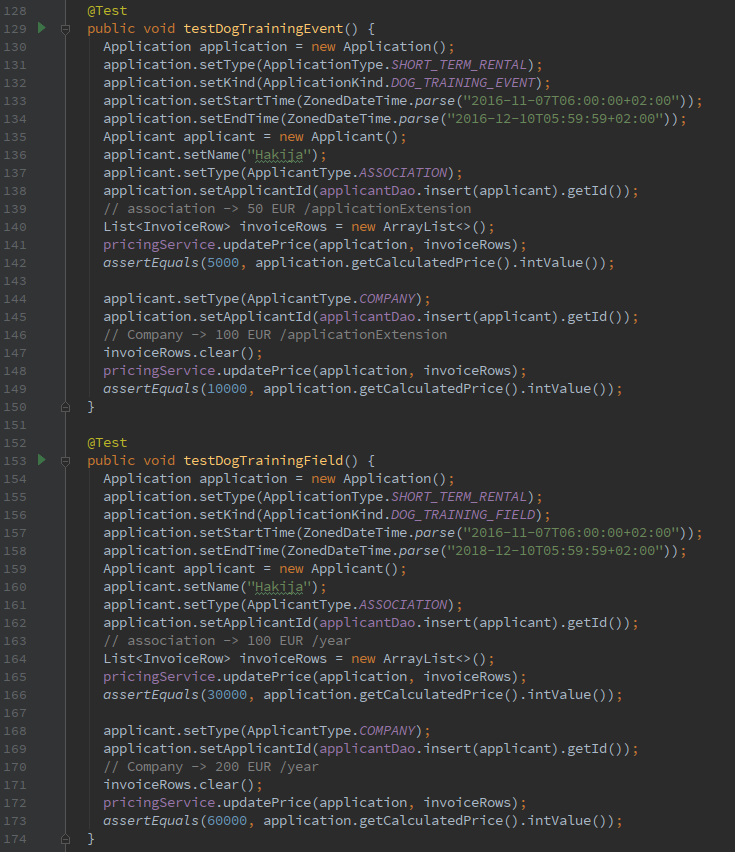
\includegraphics[width=11.0cm]{images/junit-pricing-examples.png}
        \caption{JUnit test methods to be refactored}
        \label{fig:junit-allu-refactor}
      \end{center}
    \end{figure}

    Figure \ref{fig:junit-allu-refactor} displays the example JUnit test methods. Their test run output is display in the
    figure \ref{fig:junit-allu-refactor-output}. When closely inspected, it was evident
    that the two test methods both actually included two tests inside one method which were separated by space between
    them. For example test method \textit{testDogTrainingEvent()} contains the first test within lines 130-142 and lines 144-147 are using
    the same \textit{context} of the test with modifications for a new test. At line 148 is the \textit{stimulus} of the new test and 149 holds
    the new \textit{assertion} made. Both of these test methods share mostly the same test method code and thus figures \ref{fig:spock-allu-refactor} and
    \ref{fig:spectrum-allu-refactor} display them refactored
    into tests with Spock and Spectrum that produce separate test runs with minimized repeated code.

    \begin{figure}[H]
      \begin{center}
        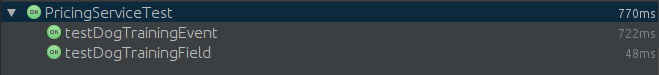
\includegraphics[width=14.7cm]{images/junit-pricing-results.png}
        \caption{JUnit test method run outputs}
        \label{fig:junit-allu-refactor-output}
      \end{center}
    \end{figure}

    \begin{figure}[H]
      \begin{center}
        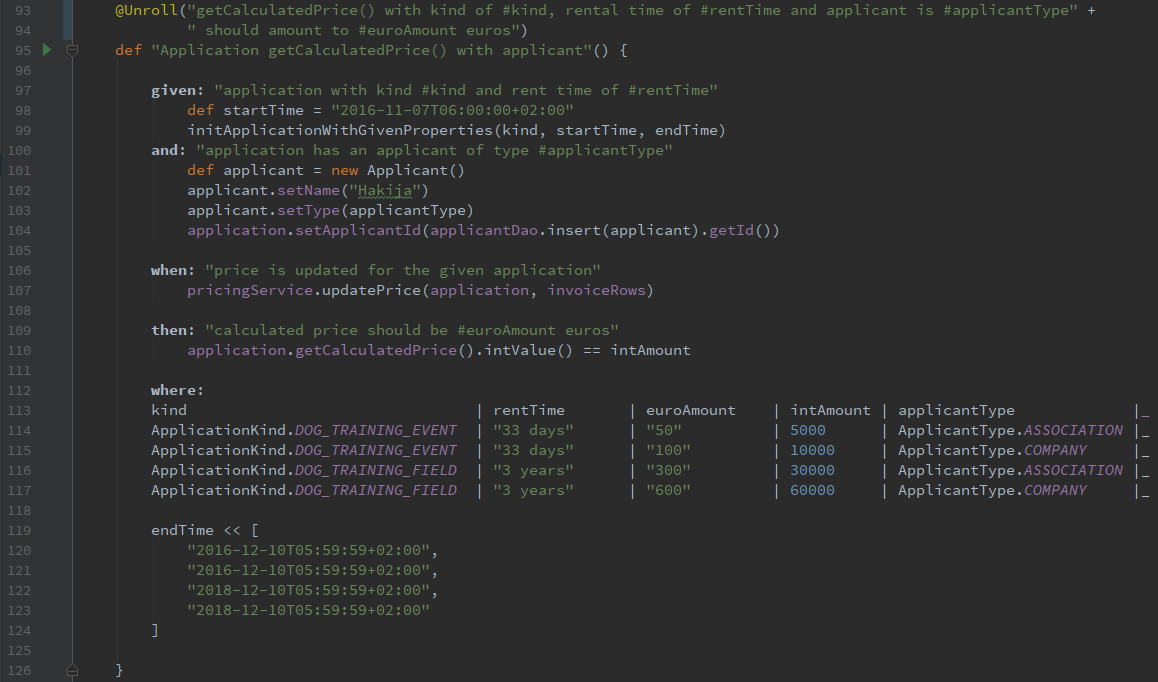
\includegraphics[width=14.7cm]{images/spock-pricing-examples.png}
        \caption{Figure \ref{fig:junit-allu-refactor} tests refactored into Spock DDT feature method}
        \label{fig:spock-allu-refactor}
      \end{center}
    \end{figure}

    In figure \ref{fig:spock-allu-refactor}, lines 112-124 together with lines 93-94 display the data driven part of a Spock
    feature method. This results in a total of
    4 separate test runs. Result of these runs in IDE can be seen in figure \ref{fig:spock-allu-refactor-output}. The
    example shows also the use of \textbf{Given-When-Then} -blocks to structure the feature method for \textit{context, stimulus}
    and \textit{assertions} together with description comments.

    \begin{figure}[H]
      \begin{center}
        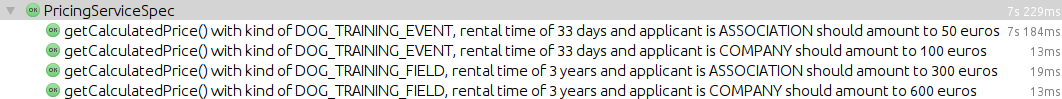
\includegraphics[width=14.7cm]{images/spock-pricing-results.png}
        \caption{Spock refactored example test run output}
        \label{fig:spock-allu-refactor-output}
      \end{center}
    \end{figure}

    \begin{figure}[H]
      \begin{center}
        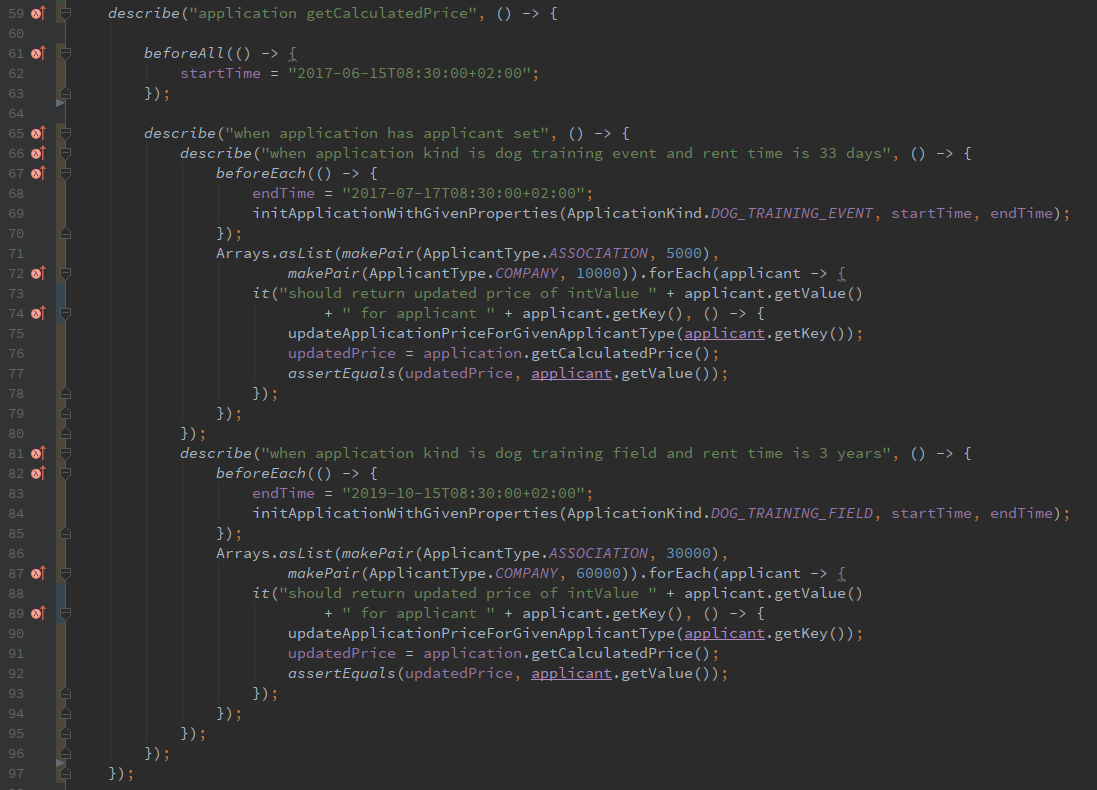
\includegraphics[width=14.7cm]{images/spectrum-pricing-examples.png}
        \caption{Figure \ref{fig:junit-allu-refactor} tests refactored into Spectrum code examples}
        \label{fig:spectrum-allu-refactor}
      \end{center}
    \end{figure}

    Figure \ref{fig:spectrum-allu-refactor} illustrates how the JUnit test methods can be refactored into Spectrum
    nested code \textbf{example groups} and \textbf{code examples}. The structure displayed in the figure produces 4 separate
    code examples. At lines 71-79 and 86-94 a custom data driven setup is made for code examples with Java 8 lambda expressions.
    All the description info from \textit{describe} and \textit{it} -blocks are concanated into test output
    that can be seen in figure \ref{fig:spectrum-allu-refactor-output}.

    \begin{figure}[H]
      \begin{center}
        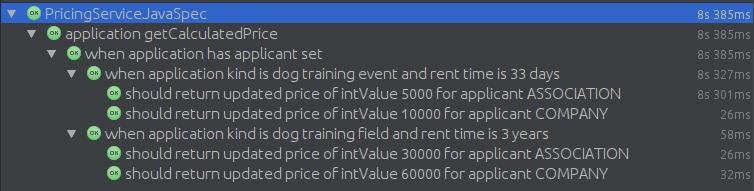
\includegraphics[width=14.7cm]{images/spectrum-pricing-results.png}
        \caption{Spectrum refactored examples test run output}
        \label{fig:spectrum-allu-refactor-output}
      \end{center}
    \end{figure}

    Altogether, the given refactored examples fit flawlessly into DDT of Spock. Spectrum test code isn't as concise in the shown example,
    but there were some other examples were Spectrum produced much less repetition than Spock for the refactored JUnit test methods.
    Both BDD testing frameworks produced \textit{separate tests} for all situations, \textit{more info on run output} and \textit{less repetition} in test code.
    After the reviewing of all refactored examples and possible positive changes against JUnit testing, project A developers chose to take
    Spectrum in use for new unit and integration test classes. Spectrum being a Java library was one the main reasons
    why developers chose it over Spock.
    \clearpage
    \subsection{Project B}
    Prior the starting of study, project B had 80 test cases/files with 465 test methods of combined automated unit and integration level tests done with JUnit.
    Current backend developer of project B had a particular DDT JUnit test case in mind that he wanted to see as a refactored example
    for Spock.

    \begin{figure}[H]
      \begin{center}
        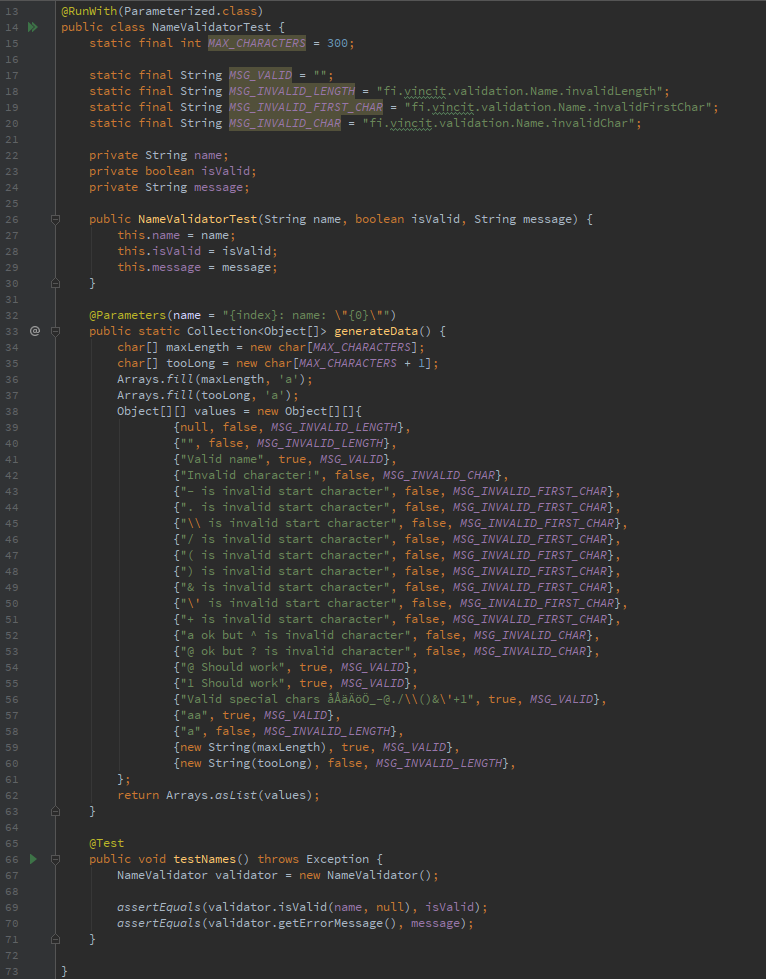
\includegraphics[width=12.7cm]{images/junit-validator-example.png}
        \caption{JUnit DDT example}
        \label{fig:junit-bit-example}
      \end{center}
    \end{figure}

    Figure \ref{fig:junit-bit-example} displays the chosen JUnit test case for refactoring. At line 13, JUnit is extended with
    \textit{Parameterized} custom runner~\cite{junit-parameterized}, which adds the DDT support for JUnit.
    Lines 26-30 and 32-63 display the creation
    of DDT test case setup in this JUnit example. At lines 65-71 is test method which uses this DDT setup. The result of running
    the test case can be seen in figure \ref{fig:junit-bit-results}.

    \begin{figure}[H]
      \begin{center}
        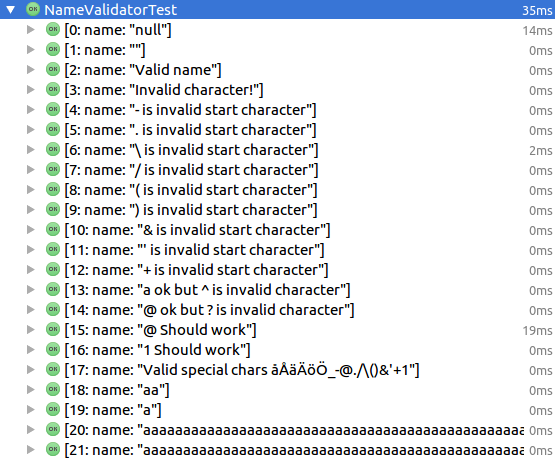
\includegraphics[width=11.7cm]{images/junit-validator-results.png}
        \caption{JUnit DDT example test run output}
        \label{fig:junit-bit-results}
      \end{center}
    \end{figure}

    Figure \ref{fig:spock-bit-example} displays the example JUnit test case refactored into Spock DDT feature method. Spock's
    data driven DSL allows to pack the same functionality into readable concise form.  At lines 37-60 the DDT table format
    is defined with \textit{where}-block and at line 24 the output of individual DDT run is defined with \textit{@Unroll}-annotation.
    The data driven parameters are used partly
    to add test output info into the feature method run. The output of feature method run can
    be seen in figure \ref{fig:junit-bit-results}.

    Compared to JUnit, Spock and its DDT feature enabled more readable and concise test structure together with more information
    containing run output. At the time of research, project B had only one developer working with JUnit testing and
    he was convinced to take Spock into use after the illustrated refactored DDT example. Spock was used in new unit and
    integration level test classes while keeping the old JUnit tests intact.

\newgeometry{bottom=1cm}
    \begin{figure}[H]
      \begin{center}
        \centerline{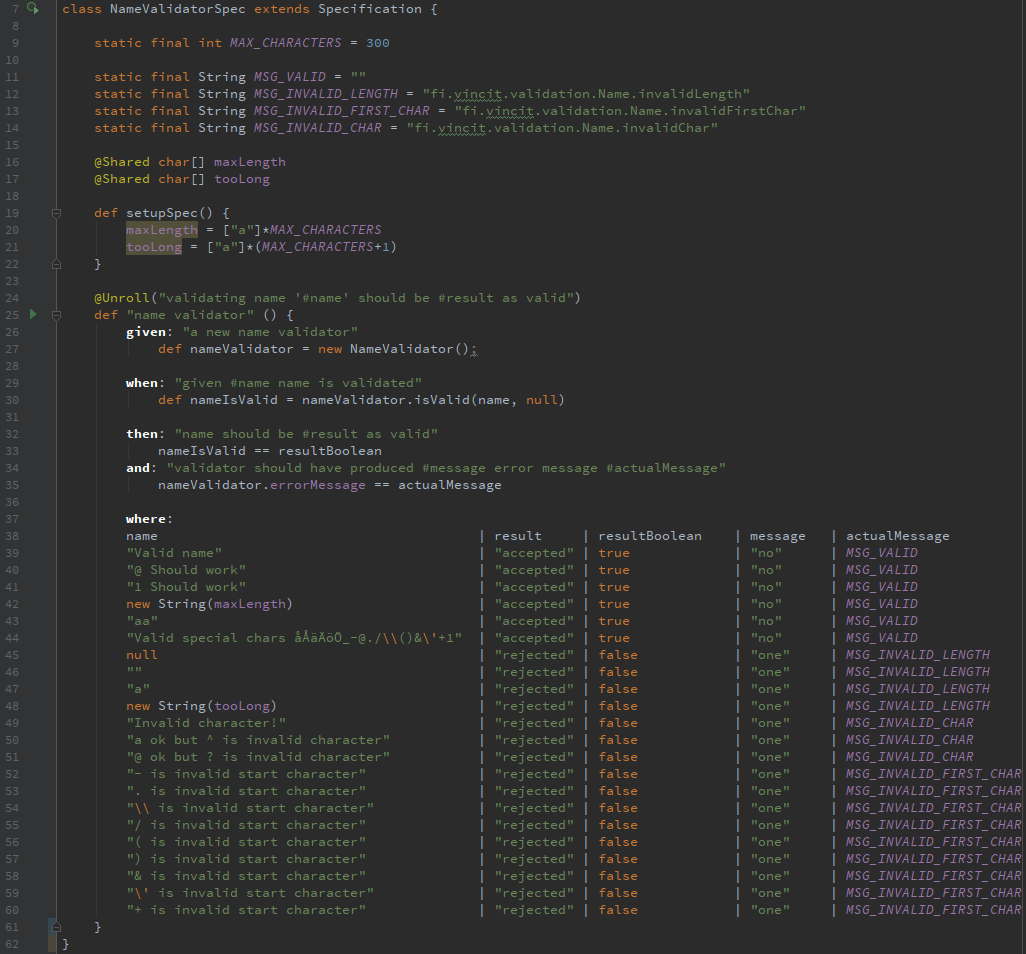
\includegraphics[width=15.7cm]{images/spock-validator-example.png}}
        \caption{Figure \ref{fig:junit-bit-example} JUnit example refactored into Spock DDT feature method}
        \label{fig:spock-bit-example}
      \end{center}
    \end{figure}

    \vspace{-38px}

    \begin{figure}[H]
      \begin{center}
        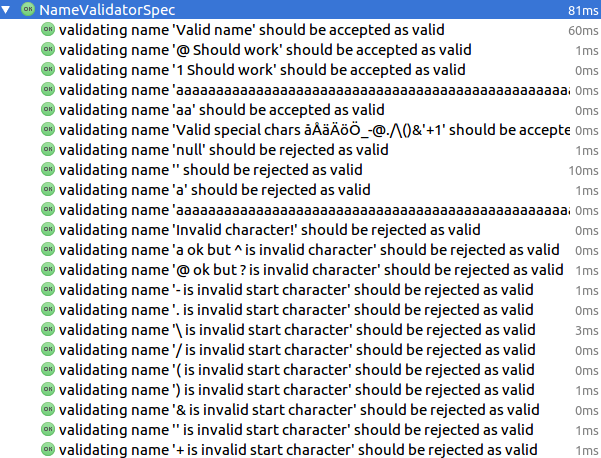
\includegraphics[width=12.7cm]{images/spock-validator-results.png}
        \caption{Spock DDT feature method run output}
        \label{fig:junit-bit-results}
      \end{center}
    \end{figure}
\restoregeometry
